\chapter{Optimized Path Planning} \label{chap:trial}
\iffalse
Keywords : 
Smooth Tour Construction with kinematic constrains,Dubins TSP,
Bezier Curve , cubic spline interpolation

bezier curve:
% http://www.joics.com/publishedpapers/2011_8_12_2441_2450.pdf

http://www.ijsce.org/attachments/File/v3i2/B1421053213.pdf
good explanation but it doesnt formulate as TSP . so refer to the book of planning and motion of UAV.


Global planner, local planner can be found  in lecture 10 planning of visual navigation for flying robots .. slide 79 before and after
The approach provided in this thesis is 2 layers of path planning. The first one is the global path planning where  the waypoints are sorted based on the shortest distance covered traversing all the given waypoints. The second layer is finding the paths between intermediate waypoints. 
This second layer can
\fi

As mentioned earlier in the previous chapter, the best waypoints to be traversed guaranteeing area coverage were chosen. Path planning algorithm should be implemented afterwards to sort these waypoints in order to assure minimal traversal 3D euclidean distance. After sorting the waypoints, there are several methods to achieve the trajectory planning that the robot should follow in between them.

This can be formally explained as 2 layer path planning consisting of global and local planners. Autonomous navigation of an aerial robot based on the combination of evolutionary algorithms as global planner, and one choice of the approaches discussed in section \ref{local_path_planning} as local planner. The use of linear piecewise function, spline piecewise function and artificial potential fields.


% The hybrid approach first uses Grid Method where the robot environment is represented by orderly numbered grids, each of which represents a location in the environment. Then, it applies Genetic Algorithm (GA), a global planner, to find an optimal path according to the current environment. The GA proposed here uses an evolutionary population initialization and genetic operators, which make the evolutionary process converge after some populations. Finally, a new Artificial Potential Field method, a local planner, is applied to follow the path obtained by GA from one intermediate node to next intermediate node avoiding the obstacles. Experimental results clearly illustrate that the proposed hybrid approach works well on large scale dynamic environments.


\textcolor{red} { hybrid PF with GA, 
http://download.springer.com/static/pdf/746/chp%253A10.1007%252F978-94-007-2792-2_31.pdf?originUrl=http%3A%2F%2Flink.springer.com%2Fchapter%2F10.1007%2F978-94-007-2792-2_31&token2=exp=1463649025~acl=%2Fstatic%2Fpdf%2F746%2Fchp%25253A10.1007%25252F978-94-007-2792-2_31.pdf%3ForiginUrl%3Dhttp%253A%252F%252Flink.springer.com%252Fchapter%252F10.1007%252F978-94-007-2792-2_31*~hmac=ec049bb412555489f79488635013bb217387263b0f56bf6ea86e6e0965c82648
}

Some operations research methods, such as traveling salesman problem (TSP), chinese postman problem and rural postman problem can be considered. In this thesis; TSP was taken into account. 


Normally path planning optimization techniques does not strictly put passing by the defined waypoint a hard constrain in their solutions. In this case hard constrains of passing by the waypoins are taken into account. A global path planner is good in producing a minimal distance path, but poor in finding intermediate waypoints and reacting to unknown obstacle.

\textcolor{red}{rectilinear environment}
so we can not rely on cell decomposition % page 7 paper carera 

\section{Global Path Planning } \label{global_path_planning}

\subsection{Problem Formulation}

% In the previous section, the method to obtain the list of waypoints has been detailed. 
% Verified by simulation that passing through all of these waypoints the desired area coverage will be attained. 

% The list of waypoints needs now to be sorted to compute an efficient path with smoother shape and shorter traveling distance. 

% \iffalse
% A process of using Dijkstra to compute an ordered list of waypoints providing shorter path. These waypoints in the sorted list is dealt with as temporary goals for the UAV to pass through. The next step is to fit the trajectory of the UAV as in \cite{curve_path}. For this waypoints are dealt as if they are graph nodes and transform the problem to be a linear or spline piecewise function .  
% \fi
% A process of formulating the problem of shortest path as traveling sales man problem and finding optimized solution using genetic algorithm is approached previously many times \textcolor{red}{citation} and validated its working principle, so it is used here in this context. The path output as ordered list of poses that guarantee the shortest path. The next step is to fit the trajectory of the UAV as in \cite{curve_path}. For this waypoints are dealt as if they are graph nodes and transform the problem to be a linear or spline piecewise function.

There are several ways to formulate this problem. In this paper, two methods have been implemented and compared.
\subsubsection{Shortest Path Problem}

Normally finding a shortest path between two points in configuration space is mature enough in research field. Dijkstra , A* and many other methods are extensively studied in the field of path planning in a grid  map inspired from graph theory \textbf{CITE}.

In our case we assume every waypoint as a goal, which define the problem as multi goal Dijkstra path planning.  So the planning in this method will simply find at every iteration the waypoint with the shortest euclidean distance from the current waypoint. Traversed waypoint will be excluded at every iteration. At the end of this process a list of ranked waypoints with the least 3D euclidean distance between every waypoint and its succedent one is obtained. This will not guarantee a globally shortest distance path.
\textcolor{red}{write in algo }
transform the area to be covered to a graph % transform the area to grid with 
discretize the graph up to a resolution needed 
assign each pose as a node in the graph
assign 3D Euclidean distance as the weight of the vertex between the nodes.

It is wide known of its slowness in the topological representation. The resolution and amount of waypoints considered as goals lead to very slow and non optimal convergence for passing by all these waypoints, so another forumaltion; as discussed in the next section shows promising results.

\subsubsection{Traveling Sales Man Problem }
The sorted path can be formulated as traveling sales man optimization problem (TSP). Every node which is a point in space (3D position) is represented as a city and the 3D euclidean distances between the cities are calculated and used as cost function. The path is organized based on the minimum distance traversing over all the waypoints. To find an optimized solution GA is here again used. The privilege of TSP problem formulation and solving it using GA over the other shortest path algorithms like Dijkstra, is that it provides global  complete solution traversing all the waypoints not finding a path from a starting node to a goal node. The GA approach for multiple waypoint path planning is more clarified and discussed by Trevor \textit{et al}. in \cite{davies2006multiple}.

The algorithm can be explained in abstract as 
\textcolor{red}{|||||||||||||||||}

1. Generate a new population of the previous population by updating all paths in the current
population. The point hereditary is determined. The path is amended by deleting the initial
points and adding other segments to reach all paths to the end point.
2. Start the algorithm for a static planning to the population and find the best path.
3. Send the best path to the aerial robot when it reached the crossing point current.
4. Update estimates of site locations for the environment.
5. Go back to step one.

Algorithm 2 Genetic Algorithm
1. Start
2. Population initialization
3. Repeat until satisfying stop criteria
4. Selection
5. Cross-over: two selected chromosomes can be combined by a cross-over operator, the result of which will replace the lowest fitness chromosome in the population. Selection of each chromosome is performed by an algorithm to ensure that the selection probability is proportional to the fitness of the chromosome. A new chromosome has the chance to be better than the replaced one. The process is oriented towards the sub-regions of the search space, where an optimalsolution is supposed to exist.
6. Mutation: a gene from the selected chromosome is randomly changed. This provides additional chances of entering unexplored sub-regions. Finally, the evolution is stopped when either the goal is reached or a maximum CPU time is reached.
7. Making new population with the fittest solutions
8. Evaluation
9. Checking the stop criteria
10. Take the best solution as output
11. End


% The privilege of GA over the Geometric Algorithms and sampling based algorithms is finding a complete solution traversing all the waypoints not finding a path from a starting node(pose) to a goal node(pose) %, not like grid or probabilistic methods used to navigate from one waypoint to another

% After having a sorted list of poses to be traversed, the next step is to fit the trajectory of the UAV as in Chang et al \cite{curve_path}.


\section{Local Path Planning} \label{local_path_planning}

After succeeding in getting the main waypoints sorted in a way to grantee shortest path distance, now comes the issue of generating the mid waypoints that the robot should traverse to generate the trajectory.


\subsection{Linear Piecewise Interpolation}
The previous process will provide a list of sorted  waypoints co-ordinates. These waypoints are dealt as graph nodes, that need to be connected to have a path, so the problem is formulated as a linear or spline piecewise function.

 Hereby the used linear piecewise function used in Eq.(\ref{eq:3}).

\begin{equation} \label{eq:3}
f(x)=
\left\lbrace
\begin{array}{ccc}
0  & \mbox{if} & x\leq a\\
\frac{x-a}{b-a} & \mbox{if} & a\leq x\leq b \\
\frac{c-x}{c-b} & \mbox{if} & b\leq x\leq c \\
1  & \mbox{if} & c\leq  x \\
\end{array}\right.  ,
\end{equation}

\noindent where the line segment between points \textit{a} and \textit{b} will be the line between every waypoint and the consecutive one. The third point is \textit{c} and depending on the number of waypoints variables will be added in the formula. Discretizing this point up to an extent will act as the sampling the path. % to form a trajectory.
\vfill 

\hfill

% \textcolor{red}{Shall i write the general equations of linear and spline piecewise fn. ?!}
% \textcolor{davidS}{????? i thing is more about ingeniery and implementation on robots }

\begin{figure}[!htb]
\minipage{0.54\textwidth}
  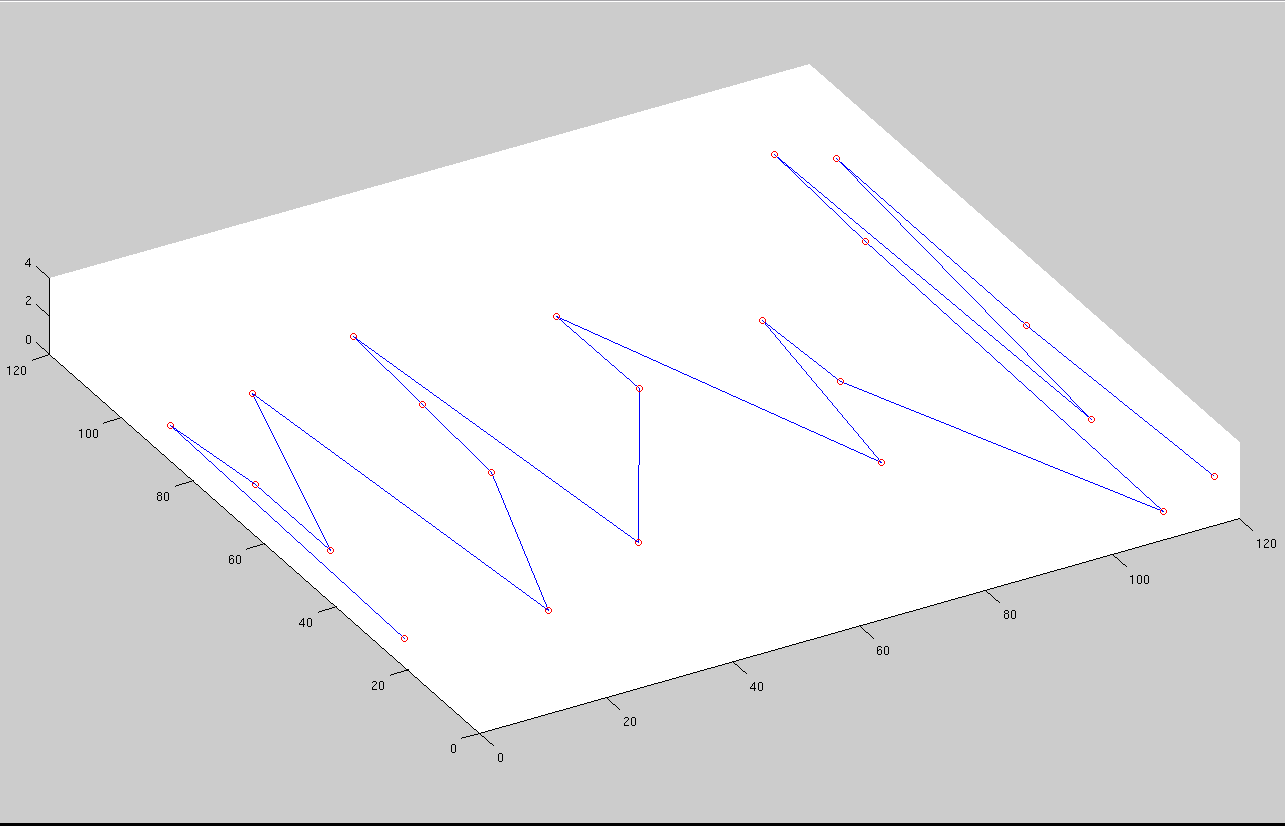
\includegraphics[width=\linewidth]{figures/DijkstraPath2.png}  
  \endminipage\hfill
  \minipage{0.45\textwidth}
   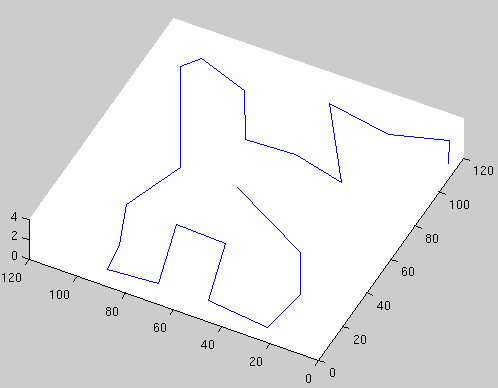
\includegraphics[width=\linewidth]{figures/Path_planned_G.png}
  \caption{Path using Dijkstra vs GA}
  \label{fig:Path_planning}
  
  \endminipage 
\end{figure}

%Traversing Distance was shorten by the 3.2 factor.  Before the path planning the distance traversed  was 166 meters and after GA applied it is nearly 51.3 meters 

The distance covered by path that is planned by GA is 513 meters which is shorter by the factor of 1.8 compared to the distance covered by Dijsktra multi goal approach which is 963 meters.

\subsection{Spline Piecewise interpolation }
% for the equation : https://en.wikipedia.org/wiki/Spline_interpolation


% REF : http://www.math.colostate.edu/~gerhard/classes/331/lab/splines.html
% http://www.sciencedirect.com/science/article/pii/0736584589900458
% Field D*: http://robots.stanford.edu/isrr-papers/final/final-23.pdf

% https://www.youtube.com/watch?v=YtcZXlKbDJY

%spline length is shorter than polynomial interpolant

The goal of the spline interpolation is to find the shortest smooth path through  consecutive waypoints. This smoothness is advisable in order to eliminate the sudden change in the first derivative or the slope of the function (line between the waypoints). It is very important as, robots specially aerial ones, require portion of time and space to change direction and rotate.

length of the interpolant = \textcolor{red}{there is a way to calculate it check }

When the interpolation is assumed to be piecewise linear, it is easy. However, if the curve is to be a spline, perhaps interpolated as a function of chordal arc length between the points, this gets a bit more difficult. A nice trick is to formulate the problem in terms of differential equations that describe the path along the curve. Then the interpolation can be done using an ordinary differential equation solver. As an example, quadcopters are considered to be holonomic. Their kinematics give hovering capabilities to these platforms. This feature permits to relax turning constraints on the path (which represents a crucial problem for fixed-wing vehicles).

\subsection{Artificial Potential Field}
It was promising idea when Artificial Potential Field (APF) was first introduced in the robotics field by Oussama Khatib in 1986 \cite{khatib1986real}. With simple rules defined in the paper as stated The manipulator moves in a field of forces. The position to be reached is an attractive pole for the end effector and obstacles are repulsive surfaces for the manipulator parts.

The procedure involves the following steps:\\
1. To establish a potential field function\\
2. to locate a minimum potential point using any optimization algorithm\\
3. to navigate an object toward the minimum potential point\\
4. to repeat steps 2 and 3 until the object reaches the goal position.\\


\begin{algorithm}
\caption{}\label{alg:euclid222}
\begin{algorithmic}[1]
\Procedure{N}{$a$}
 \State $S\gets 0$
  \While{$eval Cost(S)\leq ThresholdRate$}
	 \State $S \gets GA(NWayPoint)$
	  \State $NWayPoint\gets NWayPoint+1$
  \EndWhile\label{endwhile}
\State \textbf{return} $NWayPoint$
\EndProcedure
\end{algorithmic}
\end{algorithm}


As obstacle avoidance was the original goal of this algorithm, potential fields come with the risk of getting stuck in local minima and not being able to reach the goal. To work around this inherent characteristic one can try to formulate the potential function without local minima or incorporate techniques that allow the escape from the same, such as RRT \cite{latombe2012robot,planningBook}. In our specific case the global path planner set the initial point and the goal point provided to the APF with a guarantee to have shortest distance which will not lead to local minimum. Here APF is tweaked to only avoid the obstacles that may appear in the map, not planning the whole path.

\section{Summary}

\textcolor{red}{ the pat hplanning book 3.5.2.2 GA PF}